\documentclass[a4paper]{article}
\usepackage[utf8]{inputenc}
\usepackage[russian,english]{babel}
\usepackage[T2A]{fontenc}
\usepackage[left=10mm, top=20mm, right=18mm, bottom=15mm, footskip=10mm]{geometry}
\usepackage{indentfirst}
\usepackage{amsmath,amssymb}
\usepackage{mathastext} 
\usepackage[italicdiff]{physics}
\usepackage{graphicx}
\usepackage{caption}
\usepackage{float}
\usepackage{caption}
\renewcommand{\thefootnote}{\fnsymbol{footnote}}
\usepackage{tablefootnote}
\usepackage{footmisc}
\usepackage{textcomp}
\usepackage{multicol}
\usepackage{multirow}
\usepackage[parfill]{parskip}
\usepackage{makecell}
\usepackage{array}  
\usepackage{siunitx}
\usepackage{booktabs}
\sisetup{
    exponent-product = \cdot,
    per-mode = symbol,
    separate-uncertainty = true,
    uncertainty-separator = \,
}
\renewcommand\cellalign{cc} 
\renewcommand\cellgape{\Gape[2pt]} 
\usepackage[utf8]{inputenc}\newcommand{\approxtext}[1]{\ensuremath{\stackrel{\text{#1}}{\approx}}}
\usepackage[colorlinks=true, urlcolor=blue, linkcolor=blue, citecolor=blue]{hyperref}
\graphicspath{{images/}}
\DeclareGraphicsExtensions{.pdf,.png,.jpg}
\usepackage{wrapfig}
\captionsetup{labelformat=empty}
\usepackage{caption}
\captionsetup[figure]{name=Рисунок}
\captionsetup[table]{name=Таблица}
%\usepackage{newtxtext,newtxmath} 
\title{\textbf{Отчет о выполнении лабораторной работы 3.4.2}}
\date{}
\author{Котляров Михаил, Б01-402}

\begin{document}

\maketitle
	
\section*{Введение}

\subsection*{Цель работы}
Изучение температурной зависимости магнитной восприимчивости ферромагнетика (гадолиния) выше точки Кюри и проверка выполнения закона Кюри–Вейсса. Определение парамагнитной точки Кюри $\Theta_p$ и ферромагнитной точки Кюри $\Theta_K$.

\subsection*{Оборудование}
\begin{itemize}
    \item Катушка самоиндукции с образцом из гадолиния
    \item Термостат
    \item Частотомер
    \item Цифровой вольтметр
    \item LC-автогенератор
    \item Термопара медь–константан
\end{itemize}

\subsection*{Теоретическая часть}
Вещества с ненулевыми атомными магнитными моментами обладают парамагнитными свойствами. При повышении температуры магнитная восприимчивость парамагнетиков убывает по закону Кюри:
\[
\chi \propto \frac{1}{T}.
\]
Ферромагнетики выше температуры Кюри $\Theta_K$ подчиняются закону Кюри–Вейсса:
\[
\chi \propto \frac{1}{T - \Theta_p},
\]
где $\Theta_p$ — парамагнитная точка Кюри, близкая к $\Theta_K$.

В данной работе используется зависимость индуктивности катушки с образцом от магнитной проницаемости:
\[
L - L_0 \propto \mu - 1 = \chi,
\]
а также связь периода колебаний $LC$-генератора с индуктивностью:
\[
\tau = 2\pi \sqrt{LC}.
\]
Отсюда получаем:
\[
\chi \propto \tau^2 - \tau_0^2.
\]
Таким образом, закон Кюри–Вейсса принимает вид:
\[
\frac{1}{\tau^2 - \tau_0^2} \propto T - \Theta_p.
\]

\subsection*{Экспериментальная установка}

\begin{figure}[h]
    \centering
    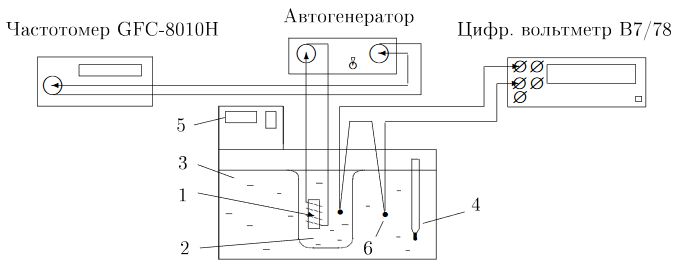
\includegraphics[scale=0.7]{Pictures/ustanovka_3_4_2.png}
    \caption{График 3. Схема экспериментальной установки.}
\end{figure}

Образец гадолиния помещён внутрь пустотелой катушки самоиндукции, которая является частью колебательного контура $LC$-автогенератора. Катушка с образцом находится в стеклянном сосуде с трансформаторным маслом, помещённом в термостат. Температура образца контролируется с помощью термопары. Период колебаний генератора измеряется частотомером.

\subsection*{Ход работы}
\begin{enumerate}
    \item Подготовим приборы к работе.
    \item Оценим допустимую ЭДС термопары при $\Delta T = 0.5^\circ\text{C}$.
\item Измерим период колебаний без образца: $\tau_0 = 6,90920$ мкс.
    \item Измерим зависимость периода колебаний $\tau$ от температуры $T$ в диапазоне от $14^\circ\text{C}$ до $40^\circ\text{C}$.

\begin{table}[h!]
    \centering
    \begin{tabular}{|c|c|c|}
        \hline
        $T$, К & $\tau$, мкс & $\frac{1}{\tau^2 - \tau_0^2}$, мкс$^{-1}$ \\ \hline
        287,10 & 7,93 & 0,0660 \\ \hline
        289,05 & 7,88 & 0,0697 \\ \hline
        291,02 & 7,80 & 0,0763 \\ \hline
        293,06 & 7,64 & 0,0941 \\ \hline
        295,04 & 7,46 & 0,1264 \\ \hline
        297,01 & 7,27 & 0,1974 \\ \hline
        299,00 & 7,15 & 0,2902 \\ \hline
        301,00 & 7,10 & 0,3688 \\ \hline
        303,06 & 7,07 & 0,4534 \\ \hline
        305,00 & 7,05 & 0,5084 \\ \hline
        307,00 & 7,03 & 0,5705 \\ \hline
        309,00 & 7,02 & 0,6302 \\ \hline
        311,00 & 7,01 & 0,6853 \\ \hline
        313,00 & 7,01 & 0,7325 \\ \hline
    \end{tabular}
    \caption{Зависимость периода колебаний контура от температуры образца}
    \label{tab:relaxation}
\end{table}

    \item Построим график зависимости $\frac{1}{\tau^2 - \tau_0^2} = f(T)$. Экстраполируем прямую к оси абсцисс и определим $\Theta_p$.
\clearpage
\begin{figure}[h]
    \centering
    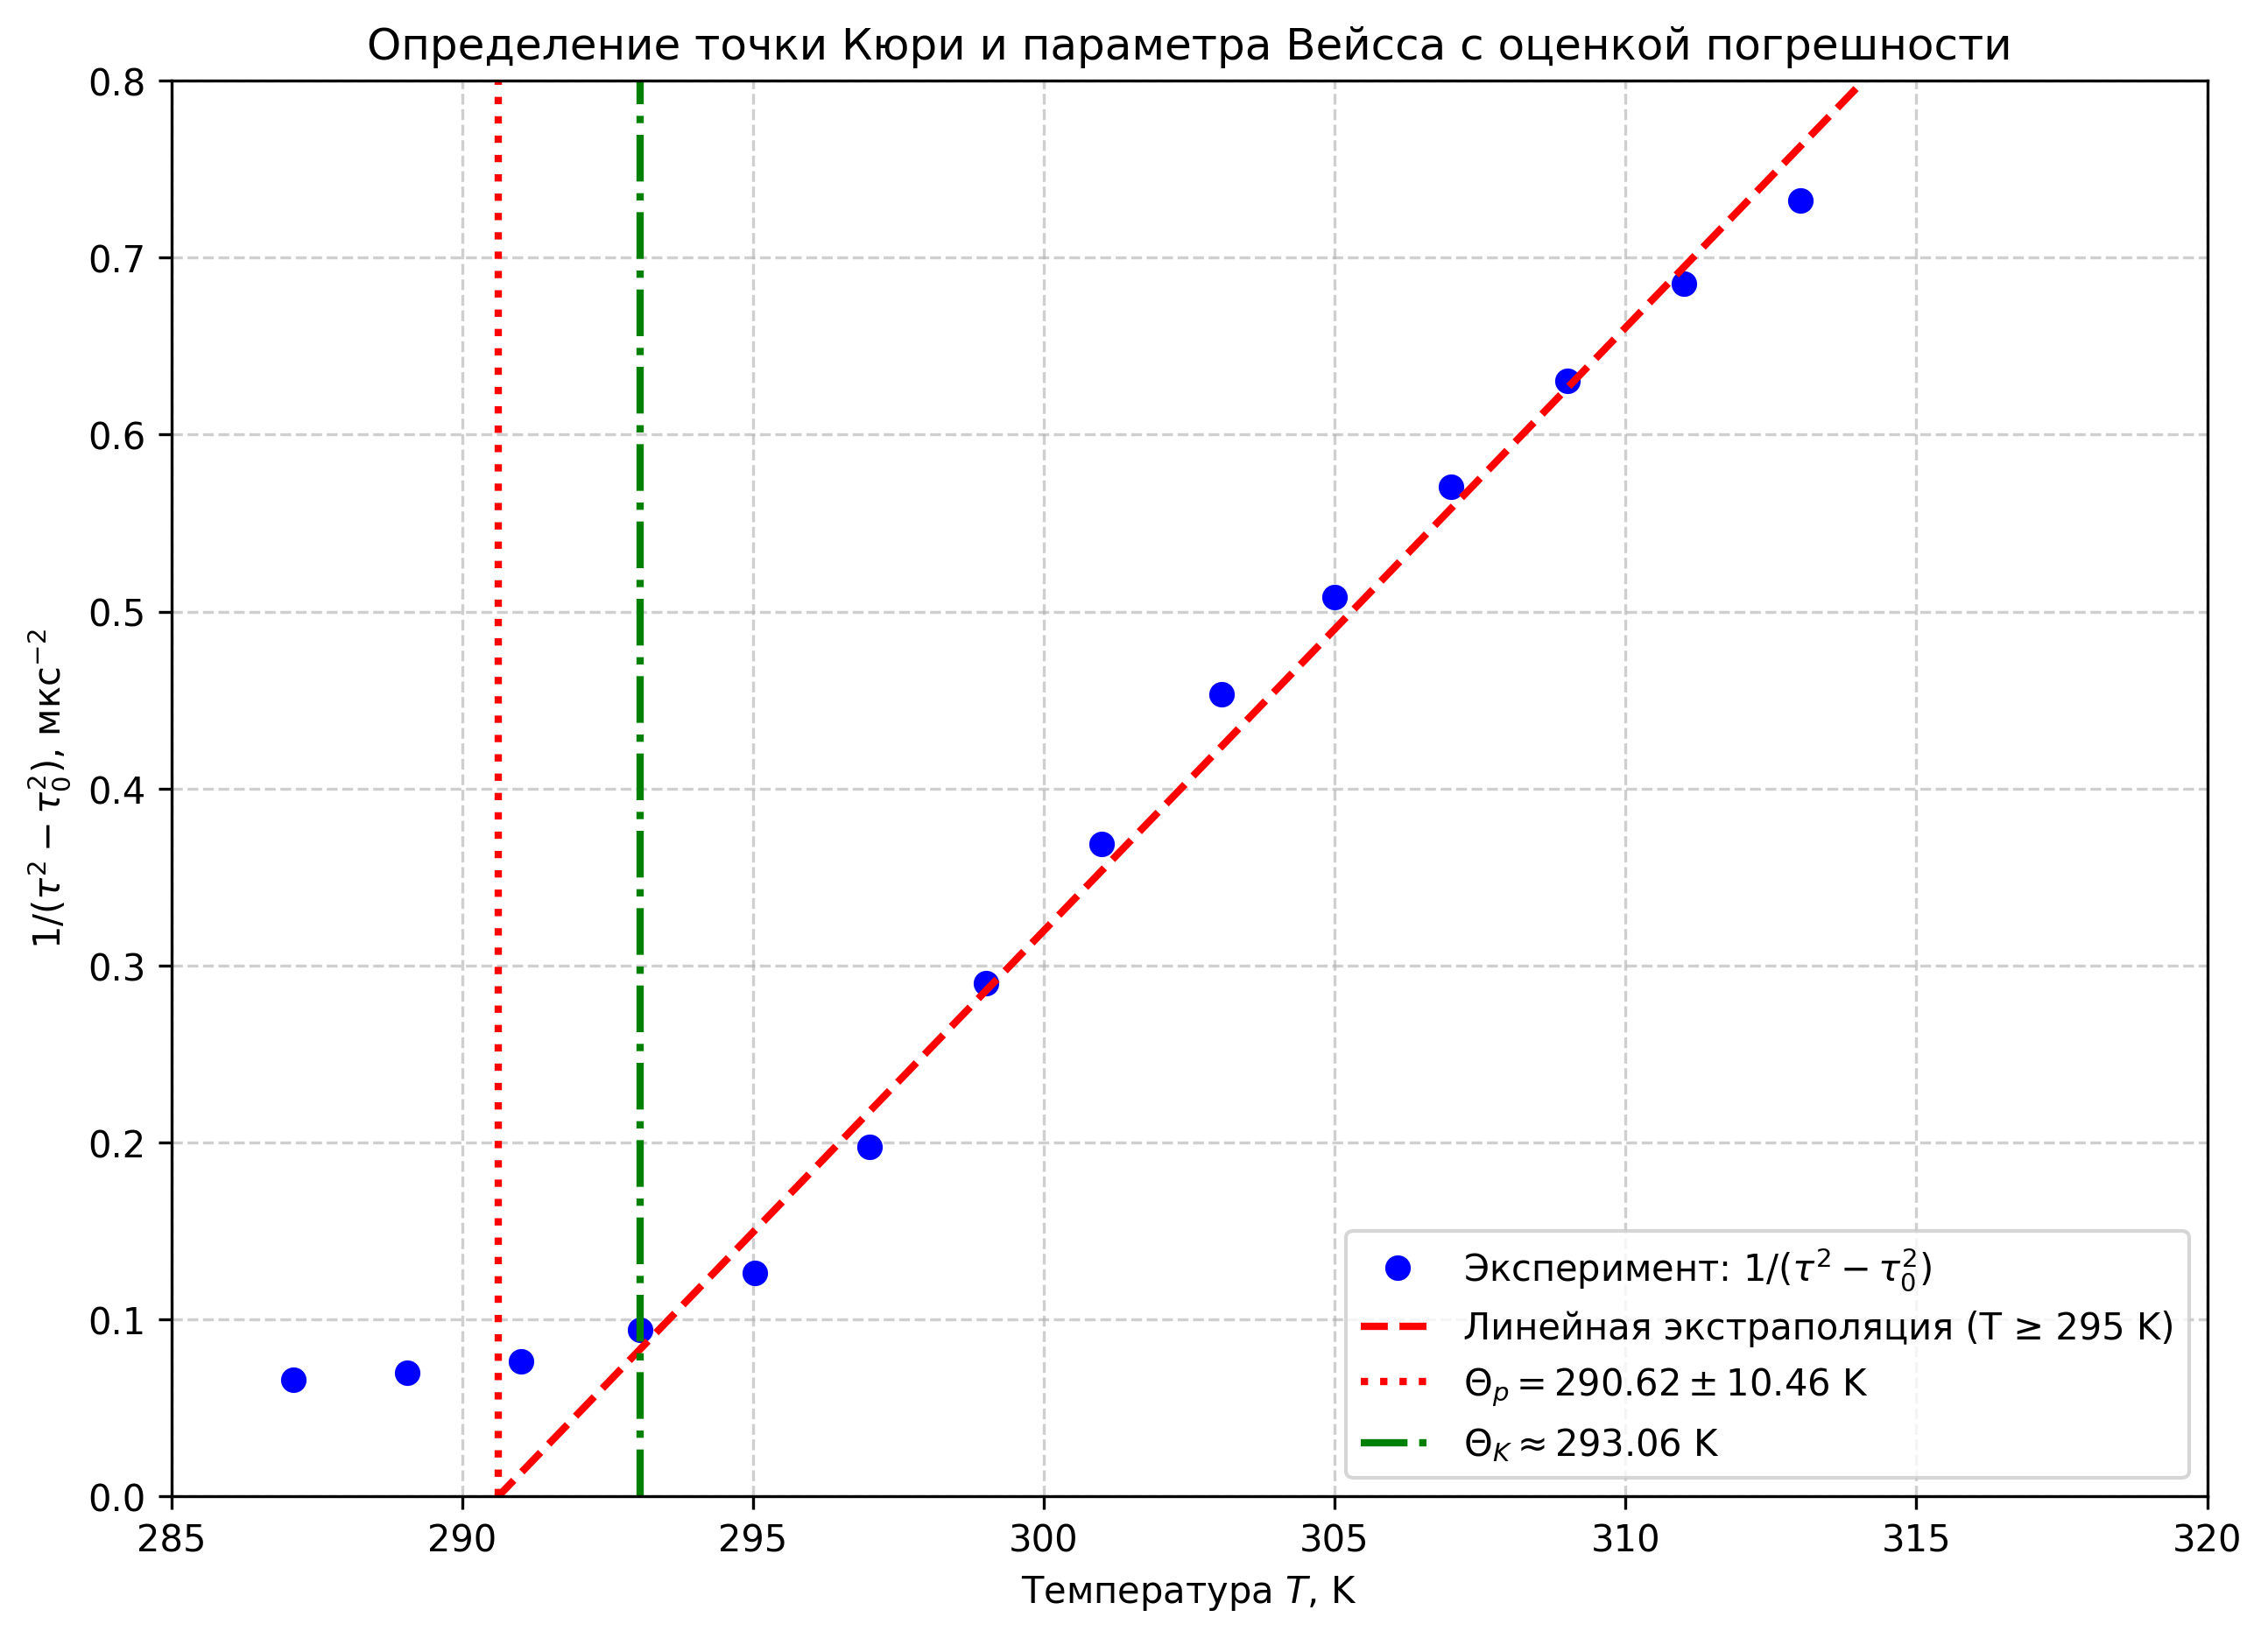
\includegraphics[scale=0.8]{Graphics/curie_point.png}
    \caption{График 1. Зависимость $\frac{1}{\tau^2 - \tau_0^2} = f(T) \propto \frac{1}{\chi}$}
\end{figure}

Получилось, что $\Theta_p = 290,62 \pm 10,46$ К, $\Theta_K \approx 293$ К.
\end{enumerate}
























\section*{Результаты и их обсуждение}

В ходе выполнения работы была исследована температурная зависимость периода колебаний $LC$-генератора с образцом гадолиния. По полученным данным построен график зависимости $\frac{1}{\tau^2 - \tau_0^2} = f(T)$, линейный участок которого аппроксимирован прямой линией.

Экстраполяция линейного участка к оси абсцисс позволила определить парамагнитную точку Кюри:
\[
\Theta_p = (290,\!62 \pm 10,\!46)\ \text{К}
\]

Анализ отклонения от линейной зависимости в области низких температур показал, что ферромагнитная точка Кюри составляет:
\[
\Theta_K \approx 293\ \text{К}
\]

Сравнение с табличным значением точки Кюри для гадолиния ($293,\!2$ К) показывает хорошее согласие в пределах погрешности:

\begin{itemize}
    \item Значение $\Theta_K$ практически совпадает с табличным (отличие менее 0,7\%)
    \item Значение $\Theta_p$ оказалось ниже табличной точки Кюри, что соответствует теоретическим представлениям
    \item Погрешность определения $\Theta_p$ составляет около 3,6\%, что является удовлетворительным результатом для данной экспериментальной установки
\end{itemize}

Различие между $\Theta_p$ и $\Theta_K$ объясняется тем, что парамагнитная точка Кюри определяется по поведению восприимчивости в парамагнитной области, в то время как ферромагнитная точка Кюри соответствует фактическому фазовому переходу.

Основными источниками погрешности могли быть:
\begin{itemize}
    \item Неидеальность теплового контакта образца с термостатом
    \item Наличие паразитных ЭДС в цепи термопары
    \item Влияние вихревых токов в образце, несмотря на его измельчение
    \item Погрешности измерения периода колебаний и температуры
\end{itemize}

\section*{Выводы}

\begin{enumerate}
    \item Экспериментально исследована температурная зависимость магнитной восприимчивости гадолиния выше точки Кюри
    \item Подтверждён закон Кюри–Вейсса для ферромагнетика в парамагнитной области
    \item Определена парамагнитная точка Кюри: $\Theta_p = (290,\!62 \pm 10,\!46)$ К
    \item Оценена ферромагнитная точка Кюри: $\Theta_K \approx 293$ К
    \item Полученные значения хорошо согласуются с табличными данными для гадолиния
\end{enumerate}
\end{document}